\documentclass[11pt]{article}

\usepackage[utf8]{inputenc}
\usepackage[T1]{fontenc}
\usepackage[spanish,es-noquoting]{babel}
\usepackage{lmodern}
\usepackage{graphicx}
\usepackage{booktabs}
\usepackage{amsmath}
\usepackage[margin=2.6cm]{geometry}
\usepackage[hidelinks]{hyperref}
\usepackage{caption}
\usepackage{float}
\usepackage{natbib}

\bibliographystyle{plainnat}
\captionsetup{font=small}

\title{\textbf{¿El modelo mira el balón o mira el césped?}\\[2mm]
\large Una auditoría con SHAP de un clasificador ViT sobre escenas de fútbol}

\author{Diego Linares\\
\small Universidad del Valle de Guatemala \\
\small Inteligencia Artificial Responsable}

\date{Septiembre de 2026}

\begin{document}
\maketitle

\begin{abstract}
\noindent
Un clasificador puede acertar la etiqueta por razones equivocadas. Este trabajo
audita un Vision Transformer preentrenado en ImageNet-1k \citep{dosovitskiy2021image}
sobre tres fotografías de fútbol que varían únicamente en cuánto contexto rodea al
objeto que nombra la clase, y pregunta si la evidencia que sostiene la predicción
\texttt{soccer ball} se concentra en el balón o se apoya en el escenario correlacionado
(césped, jugadores, gradería). Se calculan atribuciones SHAP con un explicador
agnóstico al modelo y, en lugar de interpretarlas mirándolas, se las somete a dos
pruebas que pueden refutarlas: una curva de supresión frente a un orden aleatorio y
ablaciones que aíslan el objeto o el contexto. SHAP resulta fiel en los tres casos
--borrar píxeles según su atribución degrada la predicción mucho más rápido que
borrarlos al azar-- pero el resultado central es otro: la fracción de evidencia que
SHAP coloca sobre el balón sobreestima su papel causal en un caso y, en la escena
de partido completa, la predicción correcta se sostiene \emph{sin} el balón. La
conclusión metodológica es que la masa de atribución no es una medida de necesidad
causal, y que un mapa de calor no debería aceptarse como explicación sin una prueba
de ablación que lo acompañe.
\end{abstract}

\section{Introducción}

La pregunta que motiva este trabajo es concreta y verificable: cuando un
clasificador de imágenes responde \texttt{soccer ball} ante una escena de fútbol,
¿qué parte de la imagen sostiene esa respuesta?

La pregunta importa porque una etiqueta correcta no garantiza un mecanismo correcto.
Un modelo entrenado sobre fotografías naturales aprende regularidades del conjunto de
datos, no solo del objeto: los balones de fútbol aparecen casi siempre sobre césped,
rodeados de personas con uniforme, en planos abiertos. Si el modelo aprendió a
responder al escenario en vez de al objeto, seguirá acertando mientras el escenario
se mantenga y fallará en cuanto cambie. Es el fenómeno que \citet{geirhos2020shortcut}
llaman \emph{shortcut learning}: soluciones que funcionan en la distribución de
entrenamiento y se rompen fuera de ella. Detectarlo requiere mirar el mecanismo, no
la métrica agregada.

SHAP \citep{lundberg2017unified} es hoy la herramienta estándar para esa inspección.
Reparte la diferencia entre la predicción y una línea base entre las partes de la
entrada, apoyándose en el valor de Shapley de la teoría de juegos cooperativos
\citep{shapley1953value}. El resultado es un mapa de calor por píxel, y ahí aparece el
problema práctico que este trabajo aborda: un mapa de calor es una imagen persuasiva,
y las imágenes persuasivas invitan a creerles. \citet{adebayo2018sanity} mostraron que
mapas de saliencia visualmente convincentes pueden ser insensibles al modelo e incluso
a sus pesos; \citet{kumar2020problems} y \citet{sundararajan2020many} señalan que las
atribuciones de Shapley dependen de decisiones de diseño --sobre todo de la línea
base-- que rara vez se explicitan.

Este trabajo, por tanto, no se propone únicamente producir explicaciones SHAP, sino
someterlas a prueba. El diseño experimental mantiene fija la clase y varía una sola
cosa, el tamaño relativo del objeto dentro de la escena, a lo largo de dos órdenes de
magnitud. Sobre esas tres imágenes se calculan las atribuciones y luego se verifican
con dos procedimientos independientes. Las contribuciones son:

\begin{enumerate}
  \item Un protocolo reproducible completo: modelo preentrenado, imágenes con licencia
        libre fijadas por identificador, semillas fijas y tablas del documento
        generadas desde los resultados, no escritas a mano.
  \item Evidencia de que SHAP es fiel en el sentido de la curva de supresión en los
        tres casos.
  \item Un contraejemplo dentro del mismo experimento: en la escena de partido, la
        predicción correcta \emph{no} depende del objeto que nombra la clase, algo que
        la lectura directa del mapa de calor no revela.
\end{enumerate}

\section{Metodología}

\subsection{Modelo}

Se usa \texttt{google/vit-base-patch16-224}, un Vision Transformer ViT-B/16
\citep{dosovitskiy2021image} con clasificador de 1000 clases sobre ImageNet-1k
\citep{deng2009imagenet}. El modelo se toma tal cual, sin ajuste fino, por dos
razones. La primera es de auditoría: es la situación real de quien evalúa un modelo
de terceros del que solo puede observar entradas y salidas. La segunda es de
reproducibilidad: los pesos son públicos y versionados, así que cualquiera obtiene
exactamente el mismo modelo.

ImageNet-1k contiene la clase \texttt{soccer ball}, lo que permite formular una
pregunta explicativa sin entrenar nada. Contiene además clases que compiten en el
mismo escenario (\texttt{rugby ball}, \texttt{volleyball}, \texttt{basketball},
\texttt{ballplayer}, \texttt{scoreboard}), útiles para leer con qué se confunde el
modelo cuando la confianza cae.

\subsection{Imágenes y diseño experimental}

Las tres imágenes provienen de Wikimedia Commons bajo licencias libres (dos CC0 y una
CC BY 2.0) y están fijadas en el código por su título exacto, no por una búsqueda, de
modo que la descarga es determinista. Cada archivo se registra con autor, licencia y
suma \texttt{sha256} en \texttt{data/images/manifest.json}.

Todas se preprocesan igual: se escala el lado corto a 224 px y se recorta el centro,
sin deformar la escena. Sobre ese recorte de $224\times224$ se anotó a mano la caja
envolvente del balón, ajustada después con un umbral de color. Las tres condiciones
varían el área que ocupa el objeto:

\begin{description}
  \item[A. Close-up.] El balón llena el encuadre: \textbf{69.6\%} del área. Contexto
        casi ausente.
  \item[B. Balón en el campo.] Balón nítido sobre césped, gradería desenfocada:
        \textbf{19.9\%} del área.
  \item[C. Escena de partido.] Jugadores y árbitros entrando al campo, con el balón
        en las manos de uno de ellos: \textbf{1.1\%} del área.
\end{description}

La variable independiente es entonces el tamaño relativo del objeto, que cambia en
un factor de $63$ entre A y C, mientras la clase objetivo permanece fija.

\subsection{Atribuciones SHAP}

Se emplea el \emph{Partition explainer} de la librería \texttt{shap} con máscara de
imagen por \emph{inpainting} (\texttt{inpaint\_telea}). La elección es deliberada:
este explicador solo necesita la función de predicción, de manera que el transformer
se trata como caja negra y no se accede a sus gradientes ni a su atención. Es la
condición realista de una auditoría externa y evita atarse a la arquitectura.

Las atribuciones se calculan sobre los \emph{logits} y no sobre la salida
\emph{softmax}. Con $p = 0.997$ en el caso A la probabilidad está saturada: casi
cualquier perturbación produce un cambio numéricamente nulo y el mapa resultante se
aplana sin que eso signifique ausencia de evidencia. El presupuesto es de 2000
evaluaciones del modelo por imagen, y los tres canales RGB se suman para obtener un
único mapa por píxel.

\subsection{Cómo se verifica una explicación}

Dado que el objetivo es no creerle al mapa de calor por su aspecto, se aplican tres
medidas. Las dos últimas son las que pueden refutarlo.

\paragraph{Concentración.} Fracción de la evidencia positiva que cae dentro de la caja
del balón, dividida entre la fracción de área que esa caja ocupa. Un valor de $1$
significa que la evidencia está repartida como lo estaría por azar; valores altos, que
se concentra en el objeto.

\paragraph{Curva de supresión.} Se borran progresivamente los píxeles en orden de
atribución decreciente y se mide $p(\texttt{soccer ball})$, siguiendo la lógica de
\citet{samek2017evaluating} y \citet{petsiuk2018rise}. Si las atribuciones son fieles,
esa caída debe ser más rápida que la obtenida borrando píxeles en orden aleatorio
(promedio de tres semillas). El contenido borrado se sustituye por una versión muy
desenfocada de la propia imagen ($\sigma = 15$), que destruye la forma local sin
introducir bordes artificiales. Se reporta el área bajo cada curva: menor es mejor.

\paragraph{Ablaciones.} La prueba causal directa. \emph{Solo balón} conserva el
interior de la caja y desenfoca todo lo demás: mide si el objeto \textbf{basta}.
\emph{Sin balón} desenfoca únicamente la caja y conserva el resto: mide si el objeto
es \textbf{necesario}. Las cuatro combinaciones de respuestas distinguen una
predicción anclada en el objeto de una anclada en el escenario.

\section{Resultados}

\subsection{Predicciones}

Las tres imágenes reciben la misma etiqueta, pero con confianzas que se desploman
conforme crece el contexto (Tabla~\ref{tab:pred}).

\begin{table}[H]
\centering
% Generado por src/make_tables.py. No editar a mano.
\begin{tabular}{llrlr}
\toprule
Imagen & Clase predicha & $p$ & Segunda clase & $p$ \\
\midrule
A. Close-up & \texttt{soccer ball} & 0.997 & \texttt{golf ball} & 0.001 \\
B. Balon en el campo & \texttt{soccer ball} & 0.983 & \texttt{rugby ball} & 0.007 \\
C. Escena de partido & \texttt{soccer ball} & 0.104 & \texttt{rugby ball} & 0.084 \\
\bottomrule
\end{tabular}

\caption{Predicciones del modelo. La clase es la misma en los tres casos; la confianza
cae de $0.997$ a $0.104$ al pasar del close-up a la escena completa. En C la segunda
opción (\texttt{rugby ball}, $0.084$) está prácticamente empatada con la primera.}
\label{tab:pred}
\end{table}

El caso C merece atención: con $p = 0.104$ el modelo está esencialmente indeciso entre
\texttt{soccer ball}, \texttt{rugby ball} ($0.084$) y \texttt{volleyball} ($0.059$).
Sigue siendo la respuesta correcta, y un sistema que solo registrara la etiqueta la
contaría como acierto.

\subsection{Atribuciones}

La Figura~\ref{fig:shap} muestra los mapas. En A y B la evidencia positiva se
concentra visiblemente sobre el balón, aunque el césped circundante también aporta.
En C el panorama cambia: las regiones de mayor atribución se reparten entre los
jugadores y el campo, y el balón --pequeño, en manos del árbitro-- no domina el mapa.

\begin{figure}[H]
\centering
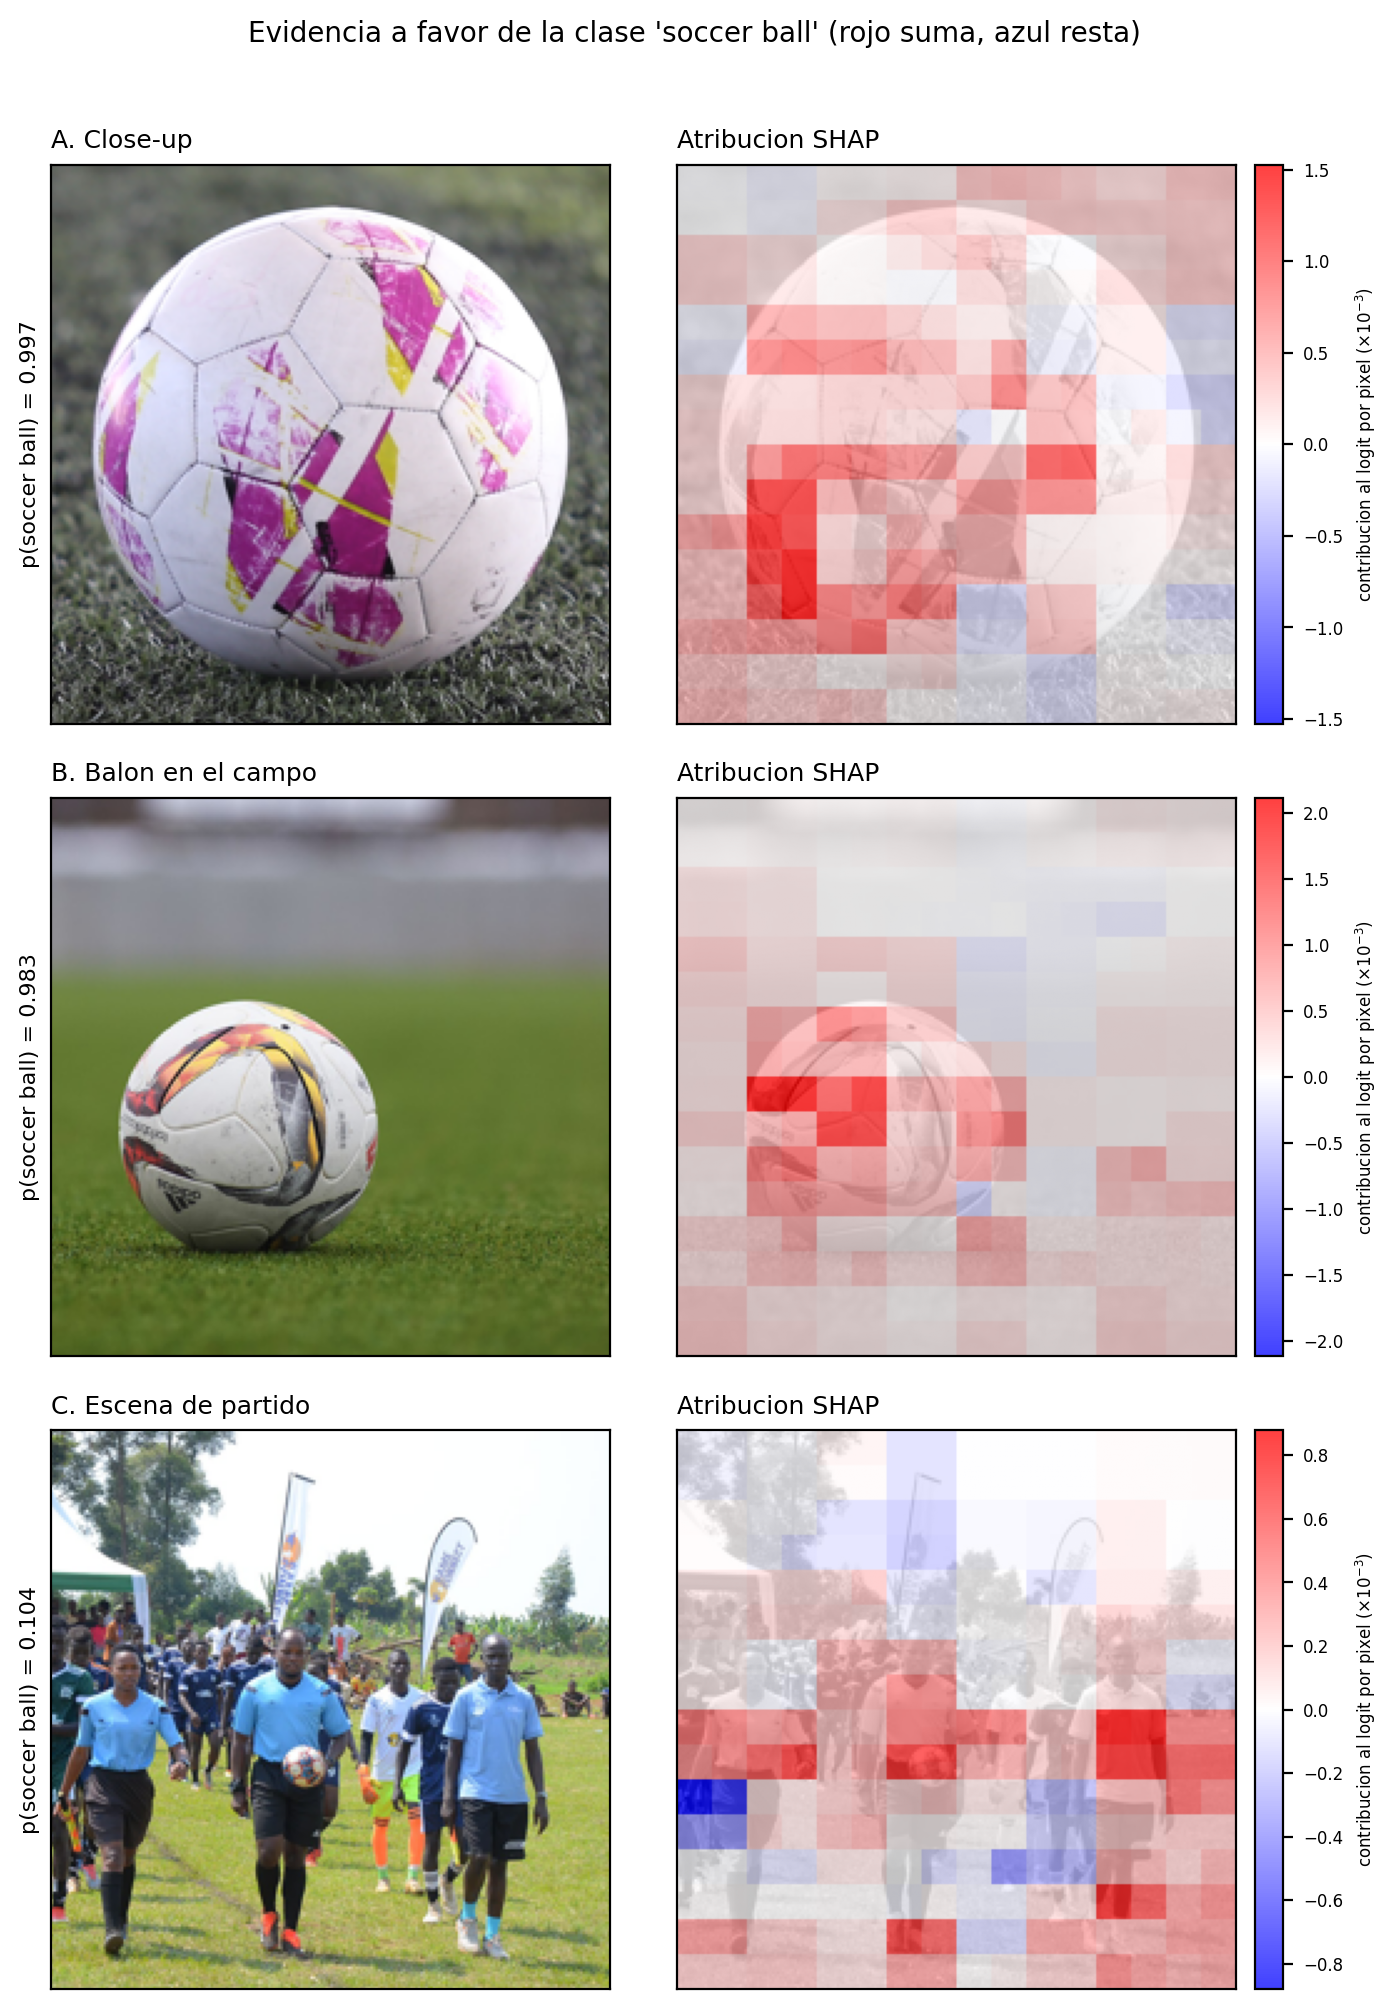
\includegraphics[width=0.82\textwidth]{../figures/shap_atribuciones.png}
\caption{Atribuciones SHAP para la clase \texttt{soccer ball}. Rojo indica píxeles que
empujan la predicción hacia la clase; azul, en contra. La resolución espacial la fija
el particionado del explicador, no el tamaño del píxel.}
\label{fig:shap}
\end{figure}

\subsection{Verificación}

\begin{table}[H]
\centering
\small
% Generado por src/make_tables.py. No editar a mano.
\begin{tabular}{lrrrrrrr}
\toprule
& \multicolumn{3}{c}{Concentracion} & \multicolumn{2}{c}{AUC supresion} & \multicolumn{2}{c}{Ablacion} \\
\cmidrule(lr){2-4} \cmidrule(lr){5-6} \cmidrule(lr){7-8}
Imagen & Area & Masa & Enriq. & SHAP & Azar & Solo balon & Sin balon \\
& (\%) & (\%) & ($\times$) & & & $p$ & $p$ \\
\midrule
A. Close-up & 69.6 & 83.4 & 1.2 & 0.291 & 0.704 & 0.994 & 0.020 \\
B. Balon en el campo & 19.9 & 53.1 & 2.7 & 0.108 & 0.294 & 0.865 & 0.001 \\
C. Escena de partido & 1.1 & 3.5 & 3.2 & 0.021 & 0.042 & 0.009 & 0.058 \\
\bottomrule
\end{tabular}

\caption{Métricas de verificación. \emph{Área}: porcentaje de la imagen ocupado por la
caja del balón. \emph{Masa}: porcentaje de la evidencia positiva que cae dentro de esa
caja. \emph{Enriq.}: cociente entre ambas. \emph{AUC supresión}: área bajo la curva de
borrado guiado por SHAP frente a borrado aleatorio; menor indica atribuciones más
fieles. \emph{Ablación}: probabilidad al conservar solo el balón y al borrar solo el
balón.}
\label{tab:metricas}
\end{table}

\paragraph{SHAP es fiel.} En las tres imágenes el AUC del borrado guiado es
sustancialmente menor que el del aleatorio ($0.291$ vs.\ $0.704$; $0.108$ vs.\ $0.294$;
$0.021$ vs.\ $0.042$). La Figura~\ref{fig:curvas} lo muestra: en A basta borrar el
$20\%$ de los píxeles mejor puntuados para que la confianza pase de $0.997$ a $0.413$,
mientras que borrar ese mismo $20\%$ al azar la deja en $0.996$. Las atribuciones
señalan píxeles que de verdad sostienen la predicción, y no se trata de un artefacto
del borrado.

\begin{figure}[H]
\centering
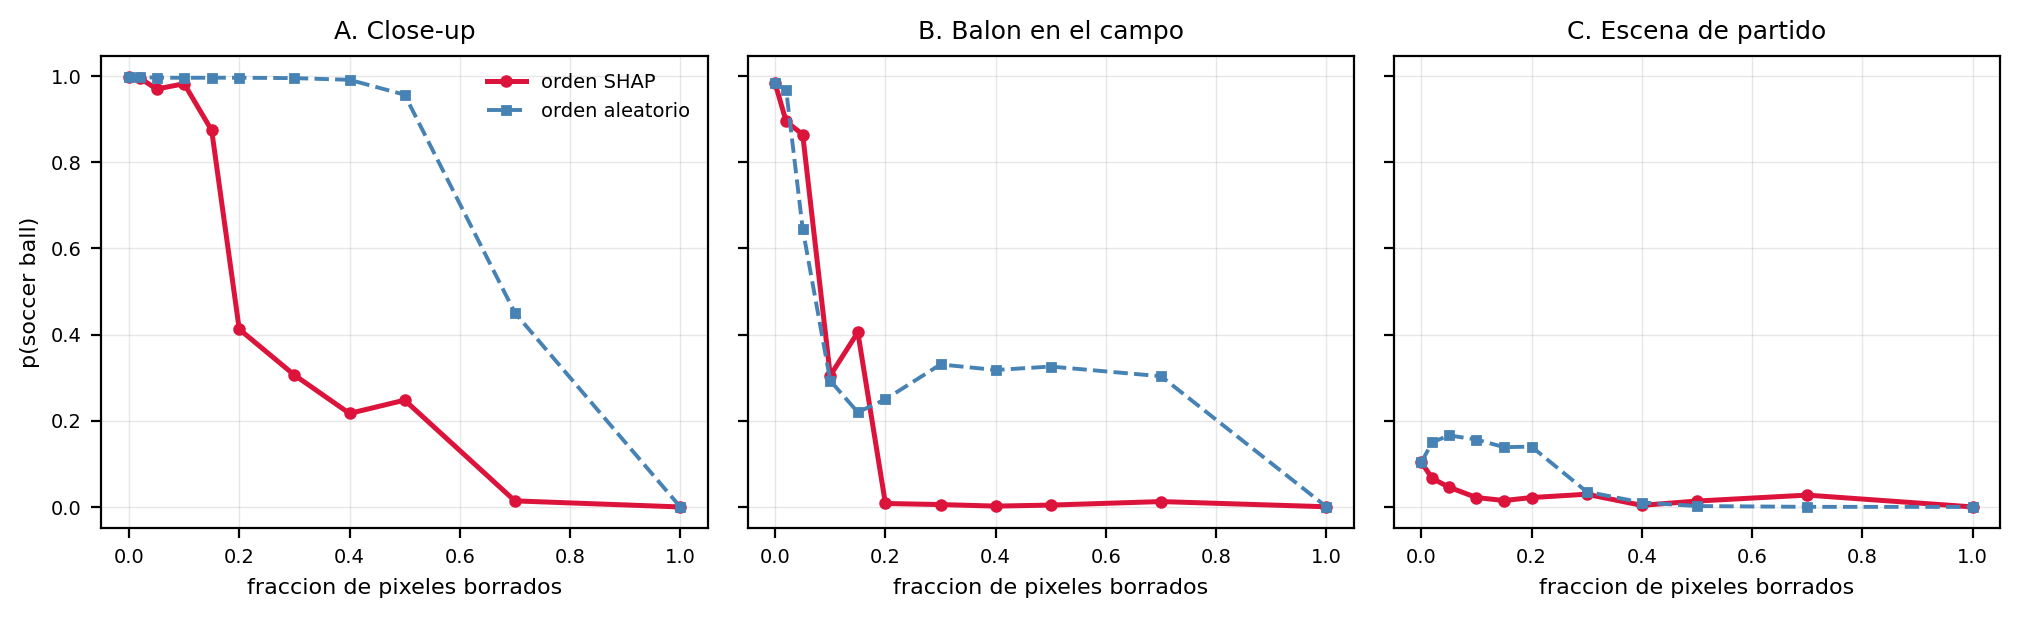
\includegraphics[width=\textwidth]{../figures/curvas_supresion.png}
\caption{Curvas de supresión. La caída más rápida del orden SHAP (rojo) frente al
aleatorio (azul) es la prueba de fidelidad. En C el orden aleatorio \emph{sube} por
encima de la confianza original, señal de lo inestable que es esa predicción.}
\label{fig:curvas}
\end{figure}

\paragraph{La concentración es modesta.} El enriquecimiento va de $1.2$ a $3.2$. En B,
el $46.9\%$ de la evidencia positiva cae \emph{fuera} del balón pese a que el objeto
es nítido y central. Leído sin más, esto sugiere que casi la mitad del sustento de la
predicción proviene del contexto.

\paragraph{Pero la masa de atribución no equivale a necesidad causal.} Las ablaciones
corrigen esa lectura. En B, borrar todo el contexto y dejar únicamente el balón apenas
mueve la predicción ($0.983 \rightarrow 0.865$), mientras que borrar solo el balón la
aniquila ($0.983 \rightarrow 0.001$). El objeto es a la vez casi suficiente y
estrictamente necesario, aunque SHAP hubiera repartido casi la mitad de la evidencia
fuera de él. El caso A se comporta igual: $0.994$ conservando solo el balón, $0.020$
borrándolo.

\paragraph{El contraejemplo.} En C el patrón se invierte. Conservar solo el balón deja
$p = 0.009$: el objeto \emph{no basta}. Y borrar el balón deja $p = 0.058$, apenas por
debajo del $0.104$ original: el objeto \emph{tampoco es necesario}. La predicción
correcta se sostiene sobre el escenario --césped, uniformes, disposición de la
escena--, no sobre el objeto que la etiqueta nombra. A esto se suma que el borrado
aleatorio \emph{aumenta} la confianza hasta $0.166$, un comportamiento que no cabe
esperar de una predicción bien fundamentada.

La Figura~\ref{fig:ablaciones} hace visible el contraste. En la fila C, la imagen que
conserva el balón es un borrón del que el modelo ya no extrae nada, mientras que la que lo
ha borrado sigue siendo una escena de fútbol perfectamente legible --- y es esa, no la
primera, la que sostiene la predicción.

\begin{figure}[H]
\centering
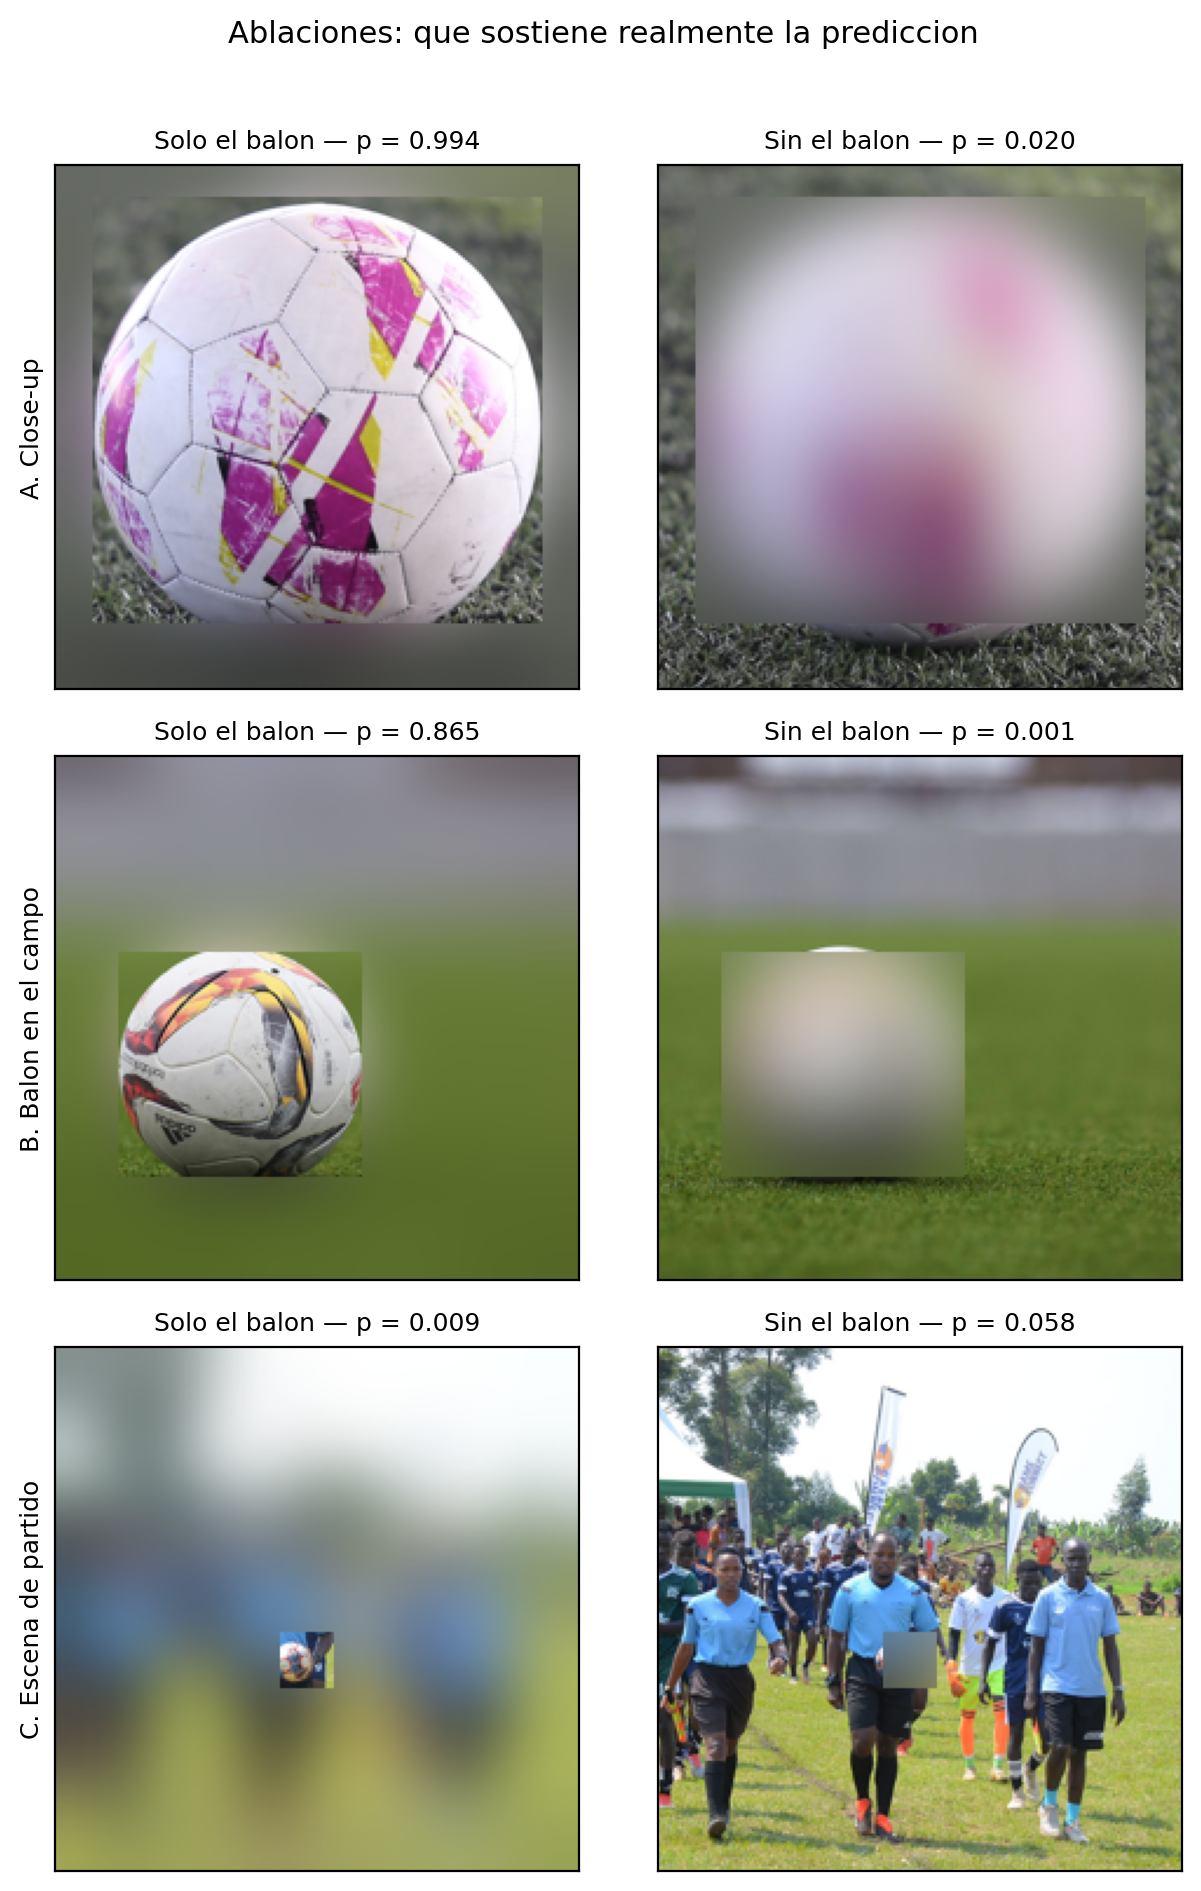
\includegraphics[width=0.66\textwidth]{../figures/ablaciones.png}
\caption{Ablaciones. Izquierda: solo se conserva la caja del balón (¿basta el objeto?).
Derecha: solo se borra la caja del balón (¿es necesario?). En A y B el objeto manda; en C
la predicción sobrevive sin él y se desploma sin el contexto.}
\label{fig:ablaciones}
\end{figure}

\section{Discusión}

\subsection{Acertar por las razones equivocadas}

El caso C es exactamente el escenario que preocupa en una auditoría: la etiqueta es
correcta, cualquier métrica agregada la contaría como acierto, y sin embargo el
mecanismo que la produce no es el que el nombre de la clase sugiere. Con el balón
borrado el modelo mantiene su respuesta; con solo el balón visible la abandona. Lo
que está reconociendo es una escena de fútbol, no un balón de fútbol.

Conviene notar que la baja confianza ($0.104$) es en sí misma una señal de alarma
disponible sin ninguna herramienta de explicabilidad. Pero la confianza sola no dice
\emph{por qué}: sin las ablaciones no habría forma de distinguir entre ``el objeto es
pequeño y difícil de ver'' y ``el objeto es irrelevante para esta predicción''. Son
diagnósticos distintos que llevan a mitigaciones distintas.

\subsection{Implicaciones para el uso de SHAP}

Tres lecciones se desprenden del experimento.

Primero, \textbf{la masa de atribución no mide necesidad causal}. En B, el $46.9\%$ de
evidencia fuera del balón invitaba a concluir que el contexto pesaba casi tanto como el
objeto; la ablación mostró que borrar todo ese contexto cuesta $0.118$ de probabilidad,
mientras que borrar el objeto cuesta $0.982$. Reportar únicamente la fracción de masa
--una práctica común-- habría producido una conclusión equivocada.

Segundo, \textbf{la fidelidad y la utilidad son propiedades distintas}. SHAP superó la
prueba de supresión en las tres imágenes, incluida C. Es decir: las atribuciones
identifican correctamente los píxeles influyentes y aun así, leídas sin ablaciones, no
delatan que la predicción de C está anclada en el contexto. Un método fiel puede
producir una explicación que se malinterpreta con facilidad.

Tercero, \textbf{la línea base es parte de la explicación}. Las atribuciones responden
a ``respecto de qué'' \citep{sundararajan2020many, kumar2020problems}: aquí, respecto de
una versión con \emph{inpainting} de la propia imagen. Otra línea base --gris uniforme,
ruido, media del conjunto-- habría dado otros números. Este trabajo la explicita, pero
no explora su sensibilidad, y esa dependencia debería declararse siempre que se reporte
un mapa SHAP.

Nada de esto contradice el valor de SHAP; sí acota cómo debe leerse. La postura de
\citet{rudin2019stop} --preferir modelos interpretables por diseño en decisiones de
alto riesgo-- gana fuerza cuando se comprueba cuánto trabajo adicional cuesta
convertir un mapa de calor en una afirmación defendible sobre el mecanismo.

\subsection{Una observación sobre la imagen C}

La escena de partido es una fotografía tomada en Uganda, en un campo comunitario. El
modelo la clasifica con una confianza diez veces menor que a las otras dos. Sería
incorrecto extraer de una sola imagen una conclusión sobre sesgo geográfico: la
diferencia de confianza se explica suficientemente por el tamaño del objeto, que es la
variable que este diseño manipula. Pero la observación conecta con un hallazgo
documentado --\citet{devries2019does} muestran que los sistemas de reconocimiento de
objetos rinden peor sobre imágenes de hogares de ingresos bajos y de países
subrepresentados en los datos de entrenamiento-- y señala la extensión natural de este
trabajo: repetir el protocolo sobre un conjunto estratificado por región y por tamaño
de objeto, donde ambos factores puedan separarse.

\section{Limitaciones}

\begin{enumerate}
  \item \textbf{Tres imágenes no son una muestra.} El diseño ilustra un mecanismo y no
        estima su frecuencia. Todo lo afirmado vale para estos tres casos.

  \item \textbf{Las ablaciones producen entradas fuera de distribución.} Una imagen
        desenfocada en un $98.9\%$ (caso C, \emph{solo balón}) no se parece a nada que
        el modelo haya visto en entrenamiento. La caída a $0.009$ mezcla dos causas:
        la ausencia de contexto y la rareza de la entrada. Por eso las comparaciones se
        hacen entre condiciones y no sobre probabilidades absolutas.

  \item \textbf{Caja envolvente, no segmentación.} La caja del balón incluye algo de
        fondo en las esquinas, lo que \emph{sobreestima} la evidencia atribuida al
        objeto. La medida de concentración es en ese sentido conservadora respecto de
        la conclusión que se defiende.

  \item \textbf{Una sola línea base.} No se exploró la sensibilidad a la máscara, que
        es el parámetro más influyente del método.

  \item \textbf{Aproximación muestreada.} Con 2000 evaluaciones por imagen, el
        \emph{Partition explainer} aproxima los valores de Shapley mediante un
        particionado jerárquico; la resolución espacial de los mapas la fija esa
        partición, no el píxel. La propiedad aditiva se verificó comparando la suma de
        atribuciones entre presupuestos de 120 y 2000 evaluaciones: coincide en las
        cuatro cifras decimales.

  \item \textbf{Sin ajuste fino.} Los resultados describen a ViT-B/16 sobre
        ImageNet-1k, no a los detectores especializados que se usan en la práctica
        para analítica deportiva.
\end{enumerate}

\section{Reproducibilidad}

Todo el material está en \texttt{https://github.com/DiegoLinares11/LoopEngineering}.
El análisis completo vive en un único cuaderno, \texttt{analisis\_shap.ipynb}, que se
ejecuta de principio a fin sin depender de ningún otro archivo del repositorio:

\begin{verbatim}
jupyter notebook analisis_shap.ipynb    # Ejecutar > Ejecutar todas las celdas
cd paper && pdflatex paper.tex && bibtex paper && pdflatex paper.tex && pdflatex paper.tex
\end{verbatim}

El cuaderno descarga las imágenes, clasifica, calcula las atribuciones, corre las tres
pruebas de verificación y escribe tanto los archivos de \texttt{results/} y
\texttt{figures/} como las dos tablas de este documento. El presupuesto de evaluaciones
es el parámetro \texttt{EVALS}: con $2000$ se obtienen los mapas aquí presentados; con
$120$ el cuaderno entero corre en menos de dos minutos, útil para comprobar la
instalación antes de la corrida definitiva.

Las semillas están fijas ($20260902$) y cada archivo JSON de resultados incluye las
versiones exactas de Python, \texttt{torch}, \texttt{transformers}, \texttt{shap} y
\texttt{numpy} con las que se produjo. Las dos tablas del documento se generan desde
esos JSON: ninguna cifra del texto se transcribió a mano, de modo que no pueden
desincronizarse del experimento. Las imágenes se identifican por su título en Commons y
por su \texttt{sha256}. El registro de la interacción con el asistente de IA que
acompañó el desarrollo está en \texttt{docs/prompt\_log.md}.

\section{Conclusión}

Se auditó un ViT-B/16 sobre tres escenas de fútbol que varían el tamaño relativo del
objeto en un factor de 63. SHAP superó la prueba de fidelidad en los tres casos, pero
esa fidelidad no impidió que su lectura directa resultara engañosa en ambos sentidos:
sobreestimó el papel del contexto donde el objeto era causalmente decisivo (caso B) y
no delató que la predicción se apoyaba en el contexto donde el objeto era irrelevante
(caso C). La diferencia solo apareció al ablacionar.

La recomendación práctica es sencilla y barata: ningún mapa de atribución debería
reportarse como explicación sin al menos una prueba de necesidad y una de suficiencia
sobre la región que señala. En este trabajo la verificación completa costó $46$ pasadas
hacia adelante por imagen --$44$ de la curva de supresión y $2$ de las ablaciones--
frente a las $2000$ que exigió el mapa de atribución. Las dos que cambiaron la
conclusión fueron esas últimas dos.

\bibliography{refs}

\end{document}
